\chapter{Introduction}
% Intro shared by all subsections

%\input{volume-1-intro/chapter-execsum} -- copied from there but heading levels changed

\section{Introduction to the \expshort Project}
\label{sec:intro-lbne-each-vol}

The \explong (\expshort) Project team has prepared this Conceptual
Design Report (CDR) which describes a world-class facility to enable a compelling research program in 
neutrino physics. The ultimate goal in
the operation of the facility and experimental program is to measure fundamental physical
parameters, explore physics beyond the Standard Model and better elucidate the nature of matter
and antimatter. 

Although the Standard Model of particle physics presents a remarkably accurate
description of the elementary particles and their interactions, it is known that the current
model is incomplete and that a more fundamental underlying theory must exist. Results from the
last decade, revealing that the three known types of neutrinos have nonzero mass, mix with one
another and oscillate between generations, point to physics beyond the Standard Model.
Measuring the mass and other properties of neutrinos is fundamental to understanding the deeper,
underlying theory and will profoundly shape our understanding of the evolution of the universe.


\subsection{About this Conceptual Design Report}
The \expshort Conceptual Design Report is intended to describe, at a conceptual level, the scope and 
design of the experimental and conventional facilities that the \expshort Project plans to build to address 
a well-defined set of neutrino-physics measurement objectives.  At this Conceptual Design stage the 
\expshort Project presents a {\em Reference Design} for all of the planned components and facilities, and 
alternative designs that are still under consideration for particular elements. 
%the science goals listed in Chapter~\ref{v1ch:sci-objectives}.  
The scope includes 
\begin{itemize}
\item an intense neutrino beam aimed at a far site
\item detectors located at the near site just downstream of the neutrino source
\item a massive neutrino detector located at the far site
\item construction of conventional facilities at both the near and far sites
\end{itemize}
The selected near and far sites are Fermi National Accelerator Laboratory (Fermilab), in Batavia, IL and  
Sanford Underground Laboratory at Homestake (Sanford Laboratory), respectively. The latter is the site of 
the formerly proposed Deep Underground Science and Engineering
Laboratory (DUSEL) in Lead, South Dakota.

This CDR is organized into six stand-alone volumes, one to describe the overall \expshort Project and one for each of its component subprojects: 
\begin{itemize}
\item Volume 1: The \expshort Project
\item Volume 2: The Beamline at the Near Site
\item Volume 3: Detectors at the Near Site
\item Volume 4: The Liquid Argon Detector at the Far Site
\item Volume 5: Cryogenic Systems
\item Volume 6: Conventional Facilities at the Near Site
\item Volume 7: Conventional Facilities at the Far Site
\end{itemize}

Volume 1 is intended to provide readers of varying backgrounds an introduction to \expshort and to the 
following volumes of this CDR.  It contains high-level information and refers the reader to topic-specific 
volumes and supporting documents, also listed in Section~\ref{intro-supp-doc}. 
Each of the other volumes contains a common, brief introduction to the overall \expshort Project, an 
introduction to the individual subproject and a detailed description of its conceptual design. 

\subsection{\expshort and the U.S. Neutrino-Physics Program}
 \hlfix{Global?}
In its 2008 report, the Particle Physics Project Prioritization Panel (P5) recommended a world-class
neutrino-physics program as a core component of the U.S. particle physics program \cite{p5report}. 
Included
in the report is the long-term vision of a large detector at the Sanford Laboratory and a high-intensity neutrino source at  Fermilab.

On January 8, 2010, the Department of Energy (DOE) approved the Mission Need for a new long-baseline
neutrino experiment that would enable this world-class program and firmly establish the
U.S. as the leader in neutrino science. The \expshort Project is designed to meet this Mission Need.

With the facilities provided by the \expshort Project, the \expshort Science Collaboration proposes to 
mount a broad attack on the science of neutrinos with sensitivity to all known parameters in a single 
experiment.  The focus of the program will be the explicit demonstration of leptonic CP violation, if it 
exists, by precisely measuring the asymmetric oscillations of muon-type neutrinos and antineutrinos into 
electron-type neutrinos and antineutrinos.

The experiment will result in the most precise measurements of the three-flavor neutrino-oscillation 
parameters over a very long baseline and a wide range of neutrino energies, in particular, the CP-
violating phase in the three-flavor framework.  The unique features of the experiment -- the long 
baseline, the broad-band beam, and the high resolution of the detector -- will enable the search for new 
physics that manifests itself as deviations from the expected three-flavor neutrino-oscillation model.

The configuration of the
\expshort facility, in which a large neutrino detector is located deep underground, could also provide
opportunities for research in other areas of physics, such as nucleon decay and neutrino
astrophysics, including studies of neutrino bursts from supernovae occuring in our galaxy. The
scientific goals and capabilities of \expshort are outlined in Volume 1 of this CDR and described fully in 
the \expshort Case Study Report
(Liquid Argon TPC Far Detector)~\cite{caseStudy} and the 2010 Interim Report of
the \explong Collaboration Physics Working Groups~\cite{PWGIReport}.



\subsection{\expshort Project Organization}
The \expshort Project Office at Fermilab is headed by the Project Manager and assisted by the Project
Engineer, Project Systems Engineer and Project Scientist. Project Office support staff include a Project Controls Manager
and supporting staff, a Financial Manager, an Environment, Safety and Health (ES\&H) Manager, a Computing Coordinator, Quality Assurance and
Risk Managers, a documentation team and administrative support. 
The Beamline, Liquid Argon Far Detector and Conventional Facilities subprojects are managed by the 
Project Office at Fermilab, while the Near Detector Complex subproject is managed by a Project Office at Los Alamos National Laboratory (LANL).

More information on Project Organization can be found in Volume~1 of this CDR. A full description of \expshort 
Project management is contained in the \expshort Project Management Plan~\cite{PMP-2453}.

\subsection{Principal Parameters of the \expshort Project}

The principal parameters of the major Project elements are given in Table~\ref{table:param-summ-fd}. 

\begin{table}[htpb]
\caption{\expshort Principal Parameters}
\label{table:param-summ-fd}
\centering
 \begin{tabular}[htbp]{|l|| p{6cm} |}
\hline
Project Element Parameter & Value  \\
\hline\hline
Near- to Far-Site Baseline &  1,300~km\\
\hline
Primary Proton Beam Power &  708~kW, upgradable to 2.3~MW\\
\hline
Protons on Target per Year &   $6.5 \times 10^{20}$  \\
\hline
Primary Beam Energy &  60 -- 120 GeV (tunable) \\
\hline
Neutrino Beam Type &  Horn-focused with decay volume\\
\hline
Neutrino Beam Energy Range &  0.5 -- 5~GeV \\ 
\hline
Neutrino Beam Decay Pipe Diameter $\times$ Length &  4~m $\times$ 200~m \\
\hline
Near Site Neutrino Detector Type & Liquid Argon Time Projection Chamber (LArTPC) Tracker \\
\hline
Near Site Neutrino Detector Active Mass &  18~ton \\
\hline
Far Detector Type &  LArTPC \\
\hline
Far Detector Active (Fiducial) Mass &  54 (40)~kton\\
\hline
Far Detector Depth &  1480~m \\
\hline
\end{tabular} 
\end{table}

\subsection{Supporting Documents}
\label{intro-supp-doc}
%\chapter{Supporting Documents}
% AH 12/30/11: Since I'm pulling this in as a chapter in vol 1 and as a subsection in section 1.1 of vols 2-6, I'm taking the chapter heading out and putting it directly into the file that inputs all the content of volume 1
A host of information related to the CDR is available in a set of supporting documents. Detailed information on risk analysis and mitigation, value engineering, ES\&H, costing, project management and other topics not directly in the design scope can be found in these documents, listed in 
Table~\ref{table:cd-1-doc-list}. Each document is numbered and stored in LBNE's document database, accessible via a username/password combination provided by the Project. Project documents stored in this database are made available to internal and external review committees through Web sites developed to support individual reviews.

%\fixme{Either need descriptions, or get rid of Description column; need to finalize table. AH}

\begin{center}
\begin{longtable}{|p{10cm}|p{4cm}|} %{|l|l|l|}
\caption{LBNE CD-1 Documents}
\label{table:cd-1-doc-list} \\
   \multicolumn{1}{p{10cm}}{\textbf{Title}} & % 2/23/12 AH tried upping col width from 5 and 2.
   \multicolumn{1}{p{4cm}}{\textbf{LBNE Doc Number(s)}} \\
\hline
\endfirsthead
Acquisition Plan & 5329 \\
\hline
Alternatives Analysis  & 4382    \\
\hline
Case Study Report; Liquid Argon TPC Detector &  3600   \\
\hline
Configuration Management Plan & 5452  \\
\hline
DOE Acquisition Strategy for LBNE & 5442 \\
\hline
Integrated Environment, Safety and Health Management Plan & 4514 \\
\hline
LAr-FD Preliminary ODH Analysis &  2478   \\
\hline
Global Science Objectives, Science Requirements and Traceback Reports &  4772   \\
\hline
Preliminary Hazard Analysis Report  &  4513  \\
\hline
Preliminary Project Execution Plan &   5443 \\
\hline
Preliminary Security Vulnerability Assessment Report & 4826 \\
\hline
Project Management Plan  & 2453    \\
\hline
Project Organization Chart & 5449    \\
\hline
Quality Assurance Plan & 2449    \\
\hline
Report on the Depth Requirements for a Massive Detector at Homestake & 0034  \\
\hline
Requirements, Beamline &  4835   \\
\hline
Requirements (Parameter Tables), Far Detector &  3747 (3383)\\
\hline
Requirements, Far Site Conventional Facilities  &   4408  \\
\hline
Requirements, Near Detectors & 5579 \\
\hline
Requirements, Near Site Conventional Facilities & 5437  \\
\hline
Risk Management Plan & 5749    \\
\hline
Value Engineering Report & 3082   \\
\hline
Work Breakdown Structure (WBS) & 4219    \\
\hline
%Cost Book List, Beamline &  http://lbne.fnal.gov/reviews/beam-costbooklist.shtml  \\
%\hline
%Cost Book List, Near Detector & http://lbne.fnal.gov/reviews/nd-costbooklist.shtml  \\
%\hline
%Cost and Schedule documents, LAr-FD &  5131  \\
%\hline
%\end{tabular} 
\end{longtable}
\end{center} %Seems funny that I need the "common/", but it works. AH

%%%%%%%%%%%%%%%%%%%%
\nomenclature{CDR}{Conceptual Design Report}
\nomenclature{CP}{charge parity}
\nomenclature{DOE}{Department of Energy}
\nomenclature{DUSEL}{Deep Underground Science and Engineering Laboratory}
\nomenclature{P5}{Particle Physics Project Prioritization Panel}


\section{Introduction to the Liquid Argon Far Detector}
\label{ch:detector}

\subsection{Overview}

The reference design Far Detector for LBNE is a liquid argon time projection chamber (LArTPC). 
The basic components of this detector type are a cryostat to contain the liquid argon (LAr), 
a TPC detection mechanism immersed in the LAr, readout electronics and
a cryogenic system to keep the LAr temperature at 89~K and maintain the required purity. 


As of 2014 the LBNE LArTPC, referred to as the LAr-FD, has been altered to consist of two massive detectors in
separate, parallel caverns, oriented end-to-end along the beam direction (roughly east-to-west), and located at the 4850 level (4850L) of the Sanford Laboratory. The fiducial mass of first one to be built will be 10 ktons, the second, 30 ktons. 
%The fiducial mass of each, as defined for neutrino-oscillation studies, is 16.3~kton and the active (instrumented) mass is 20~kton, resulting in a total active mass of 40~kton.
Figure~\ref{fig:cavern-layout-2014} %and~\ref{fig:LAr-FD-cavern} 
shows the proposed
layout of the Far Site, and Figure~\ref{fig:LAr-FD-config-cavern} shows the detector configuration.  The cavern and related conventional facilities are described in Volume 6 of this CDR.

\begin{figure}[htbp]
\centering
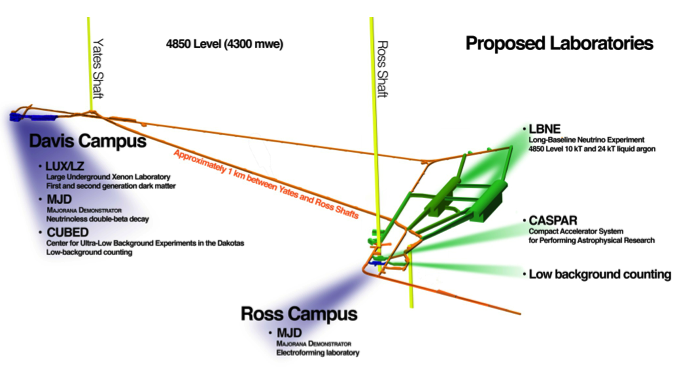
\includegraphics[width=\textwidth]{LArFD_4850L_layout_Sept25_2014.png}
\caption[Location of LAr-FD caverns at the 4850L]{Location of LAr-FD caverns at the 4850L} %(Dangermond Keane Architecture, courtesy Sanford Laboratory) 
\label{fig:cavern-layout-2014}
\end{figure}


\begin{figure}[htbp]
\centering
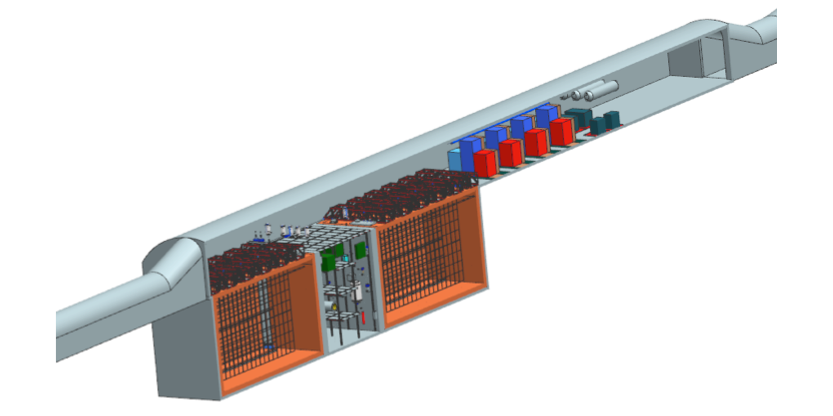
\includegraphics[width=\textwidth]{larfd-from-2794-slide9.png}
\caption[Detector configuration within the cavern]{Detector configuration within the cavern. The TPC is located within a membrane cryostat, shown in orange. 
%The interior dimensions of each cryostat are 15.6~m wide $\times$ 16~m high $\times$ 28.6~m long. The highbay is 144.3~m long and has a 18.2~m span. 
Cryogenic equipment is located at the far end of the upper cavern and the filtration equipment is in the septum area between the two cryostats. }
\label{fig:LAr-FD-config-cavern}
\end{figure}

The fiducial mass of the first is shown in Figure~\ref{fig:10kt-fiducial-mass}; a similar diagram for the second detector is not yet available.
\begin{figure}[htbp]
\centering
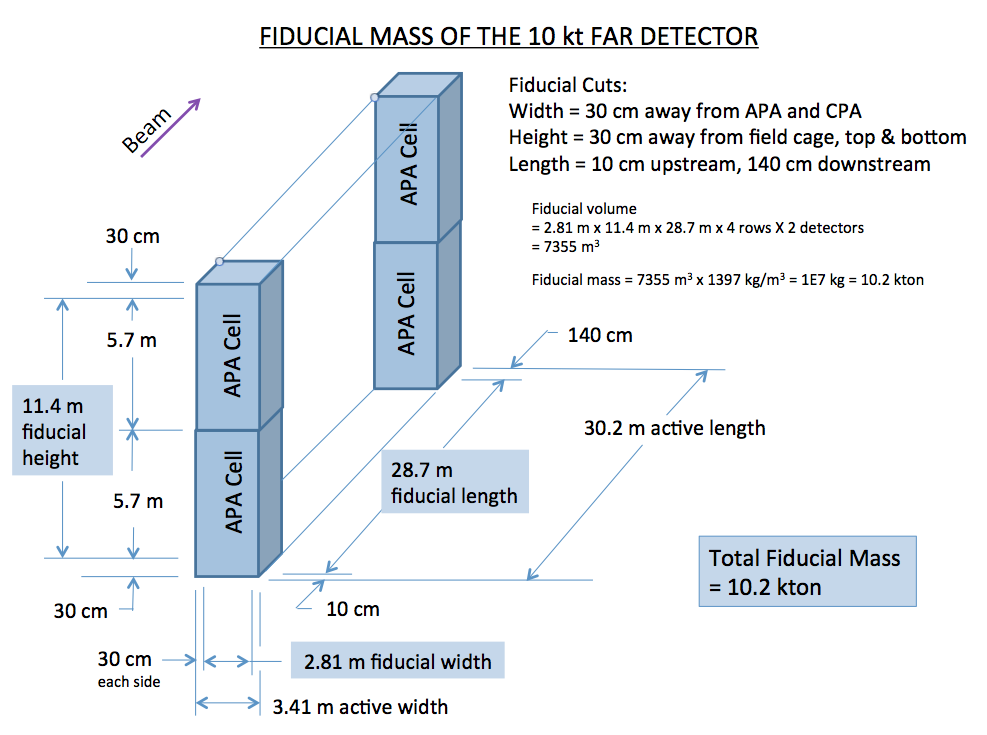
\includegraphics[width=\textwidth]{fiducial-mass-10kt-jan2015.png}
\caption[Fiducial mass of 10-kton detector]{Fiducial mass of 10-kton detector}
\label{fig:10kt-fiducial-mass}
\end{figure}

In a LArTPC, a uniform electric field is created within the TPC
volume between cathode planes and anode wire planes. Charged particles
passing through the TPC release ionization electrons that drift to the
anode wire planes. The bias voltage is set on the anode plane wires so that ionization electrons drift between the first several (induction) planes and are collected on the last (collection) plane.
Readout electronics amplify and continuously digitize
the induced waveforms on the sensing wires at several MHz, and transmit
these data to the data acquisition (DAQ)  system for processing. The wire planes are oriented at different angles allowing a 3D reconstruction of the particle trajectories. In addition to these basic
components, a photon-detection system provides a trigger for proton
decay and galactic supernova neutrino interactions. 

%%%%%%%%%%%%%%%%%%%%%%%%%%%%%%%%%%%%%%%%%%%%%%%%%%%%

The design of the LAr-FD has been developed and refined 
over the past five years. The starting point was the ICARUS  T600 system \cite{Icarus-T600}, 
and the process was informed and guided by the experience with small 
LArTPCs in the U.S., particularly ArgoNeuT~\cite{argoneut-url},  the development of designs 
for MicroBooNE~\cite{microboone-url}.
%, and by the success of the ATLAS \nomenclature{ATLAS}{A Toroidal LHC Apparatus, experiment at CERN} \nomenclature{CERN}{European Organization for Nuclear Research} LAr calorimetry~\cite{atlas-url}.  
The LAr-FD concept is designed for assembly 
%the result of an effort to assemble every major part of the detector 
from small, independent elements  which can be repeated almost indefinitely
 in any dimension to form the entire 
assembly within a large cryostat. Each 
of the elements provides an independent mechanical structure 
to support the elements it contains.  To a large extent, scaling from 
detector volumes containing anywhere from a few to 
several hundred such elements is straightforward with small 
and predictable risk. Scaling in other areas of 
LArTPC detector technology, namely cryostat construction, LAr purification
and electronics readout has been incorporated into the design.

\subsection{Cavern Layout}

\begin{editornote}
  Editor's Note: The current plan is to create space for a 40-kton detector in two separate, parallel caverns, one for 10 kton and one for 30 kton, instead of excavating a single cavern. The smaller cavern would be outfitted as soon as possible and the larger would be outfitted in a later phase of work. 
\end{editornote}


The first (smaller) LAr-FD cavern will be excavated into a ``mailbox'' cross section, as illustrated in 
Figure~\ref{fig:cavern-layout-2014}. The long axis of the cavern will point towards Fermilab, parallel to and in 
line with the neutrino beamline. The pit, the below-grade rectangular cavity inside of which the cryostats 
fit, will have dimensions %of 26.1-m wide by 18-m high by 119.2-m long.  Dimensions are 
as detailed in Figure~\ref{fig:cavern-pit-params-10kt} and illustrated in Figure~\ref{fig:v5ch2-cavern-cryostat-section-2014}.

\begin{figure}[htbp]
\centering
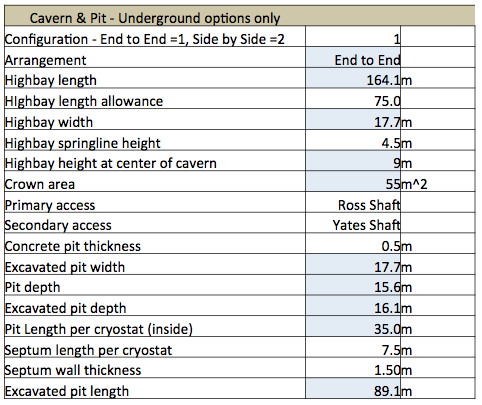
\includegraphics[width=\textwidth, angle=90]{param-10kt-cavern-and-pit.png}
\caption{Parameters for 10-kton detector cavern and pit, 2014}
\label{fig:cavern-pit-params-10kt}
\end{figure}

The parameters for the larger cavern are given in Figure~\ref{fig:cavern-pit-params-30kt}.
\begin{figure}[htbp]
\centering
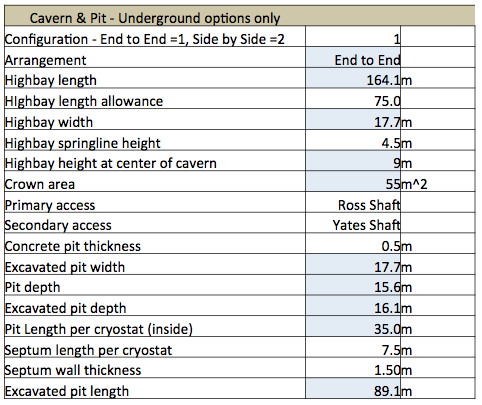
\includegraphics[width=\textwidth, angle=90]{param-10kt-cavern-and-pit.png}
\caption{Parameters for 30-kton detector cavern and pit, 2014}
\label{fig:cavern-pit-params-30kt}
\end{figure}

The 10-kton detector pit will be segmented into three 
volumes: a space for each cryostat plus a 15-m-wide clear space in the middle, called the septum,  separated from the cryostat areas by 1.5-m-thick  
walls. Equipment and vessels used for filtering LAr to achieve high purity levels will be placed in 
the septum area.  

The cavern (highbay) roof, located above the pit, will be 17.7~m wide by 164.1~m long, and its 
rounded ``mailbox top'' upper surface will arch to $\sim$10~m in the center and $\sim$5~m on the 
sides (springline). The curved upper surface will extend beyond each end of the dual-cryostat detector along the long 
axis to provide additional space for ancillary equipment as well as for installation and maintenance 
operations. 

Space will be provided for the nitrogen refrigerators, nitrogen compressors and necessary 
cryogen-storage vessels. Walkways will run the entire length of the cavern through the roof truss of the detector to 
provide personnel access along the cryostat roof. A separately ventilated emergency-egress passageway will be elevated over the roof truss section and extend to the east and west ends of the cavern highbay.

\begin{editornote}
  Editor's Note:  The illustration and dimensions in Figure~\ref{fig:v5ch2-cavern-cryostat-section-2014} are for a detector with APAs of dimensions 2.5~m $\times$ 7~m and a total of 10 adjoined end-to-end along the beamline.  The current configuration will use 2.3~m $\times$ 6~m APAs, in rows of 13 end-to-end, making the detector slightly shallower and longer than shown in the figure.  
\end{editornote}


\begin{figure}[htbp]
\centering
% 2012 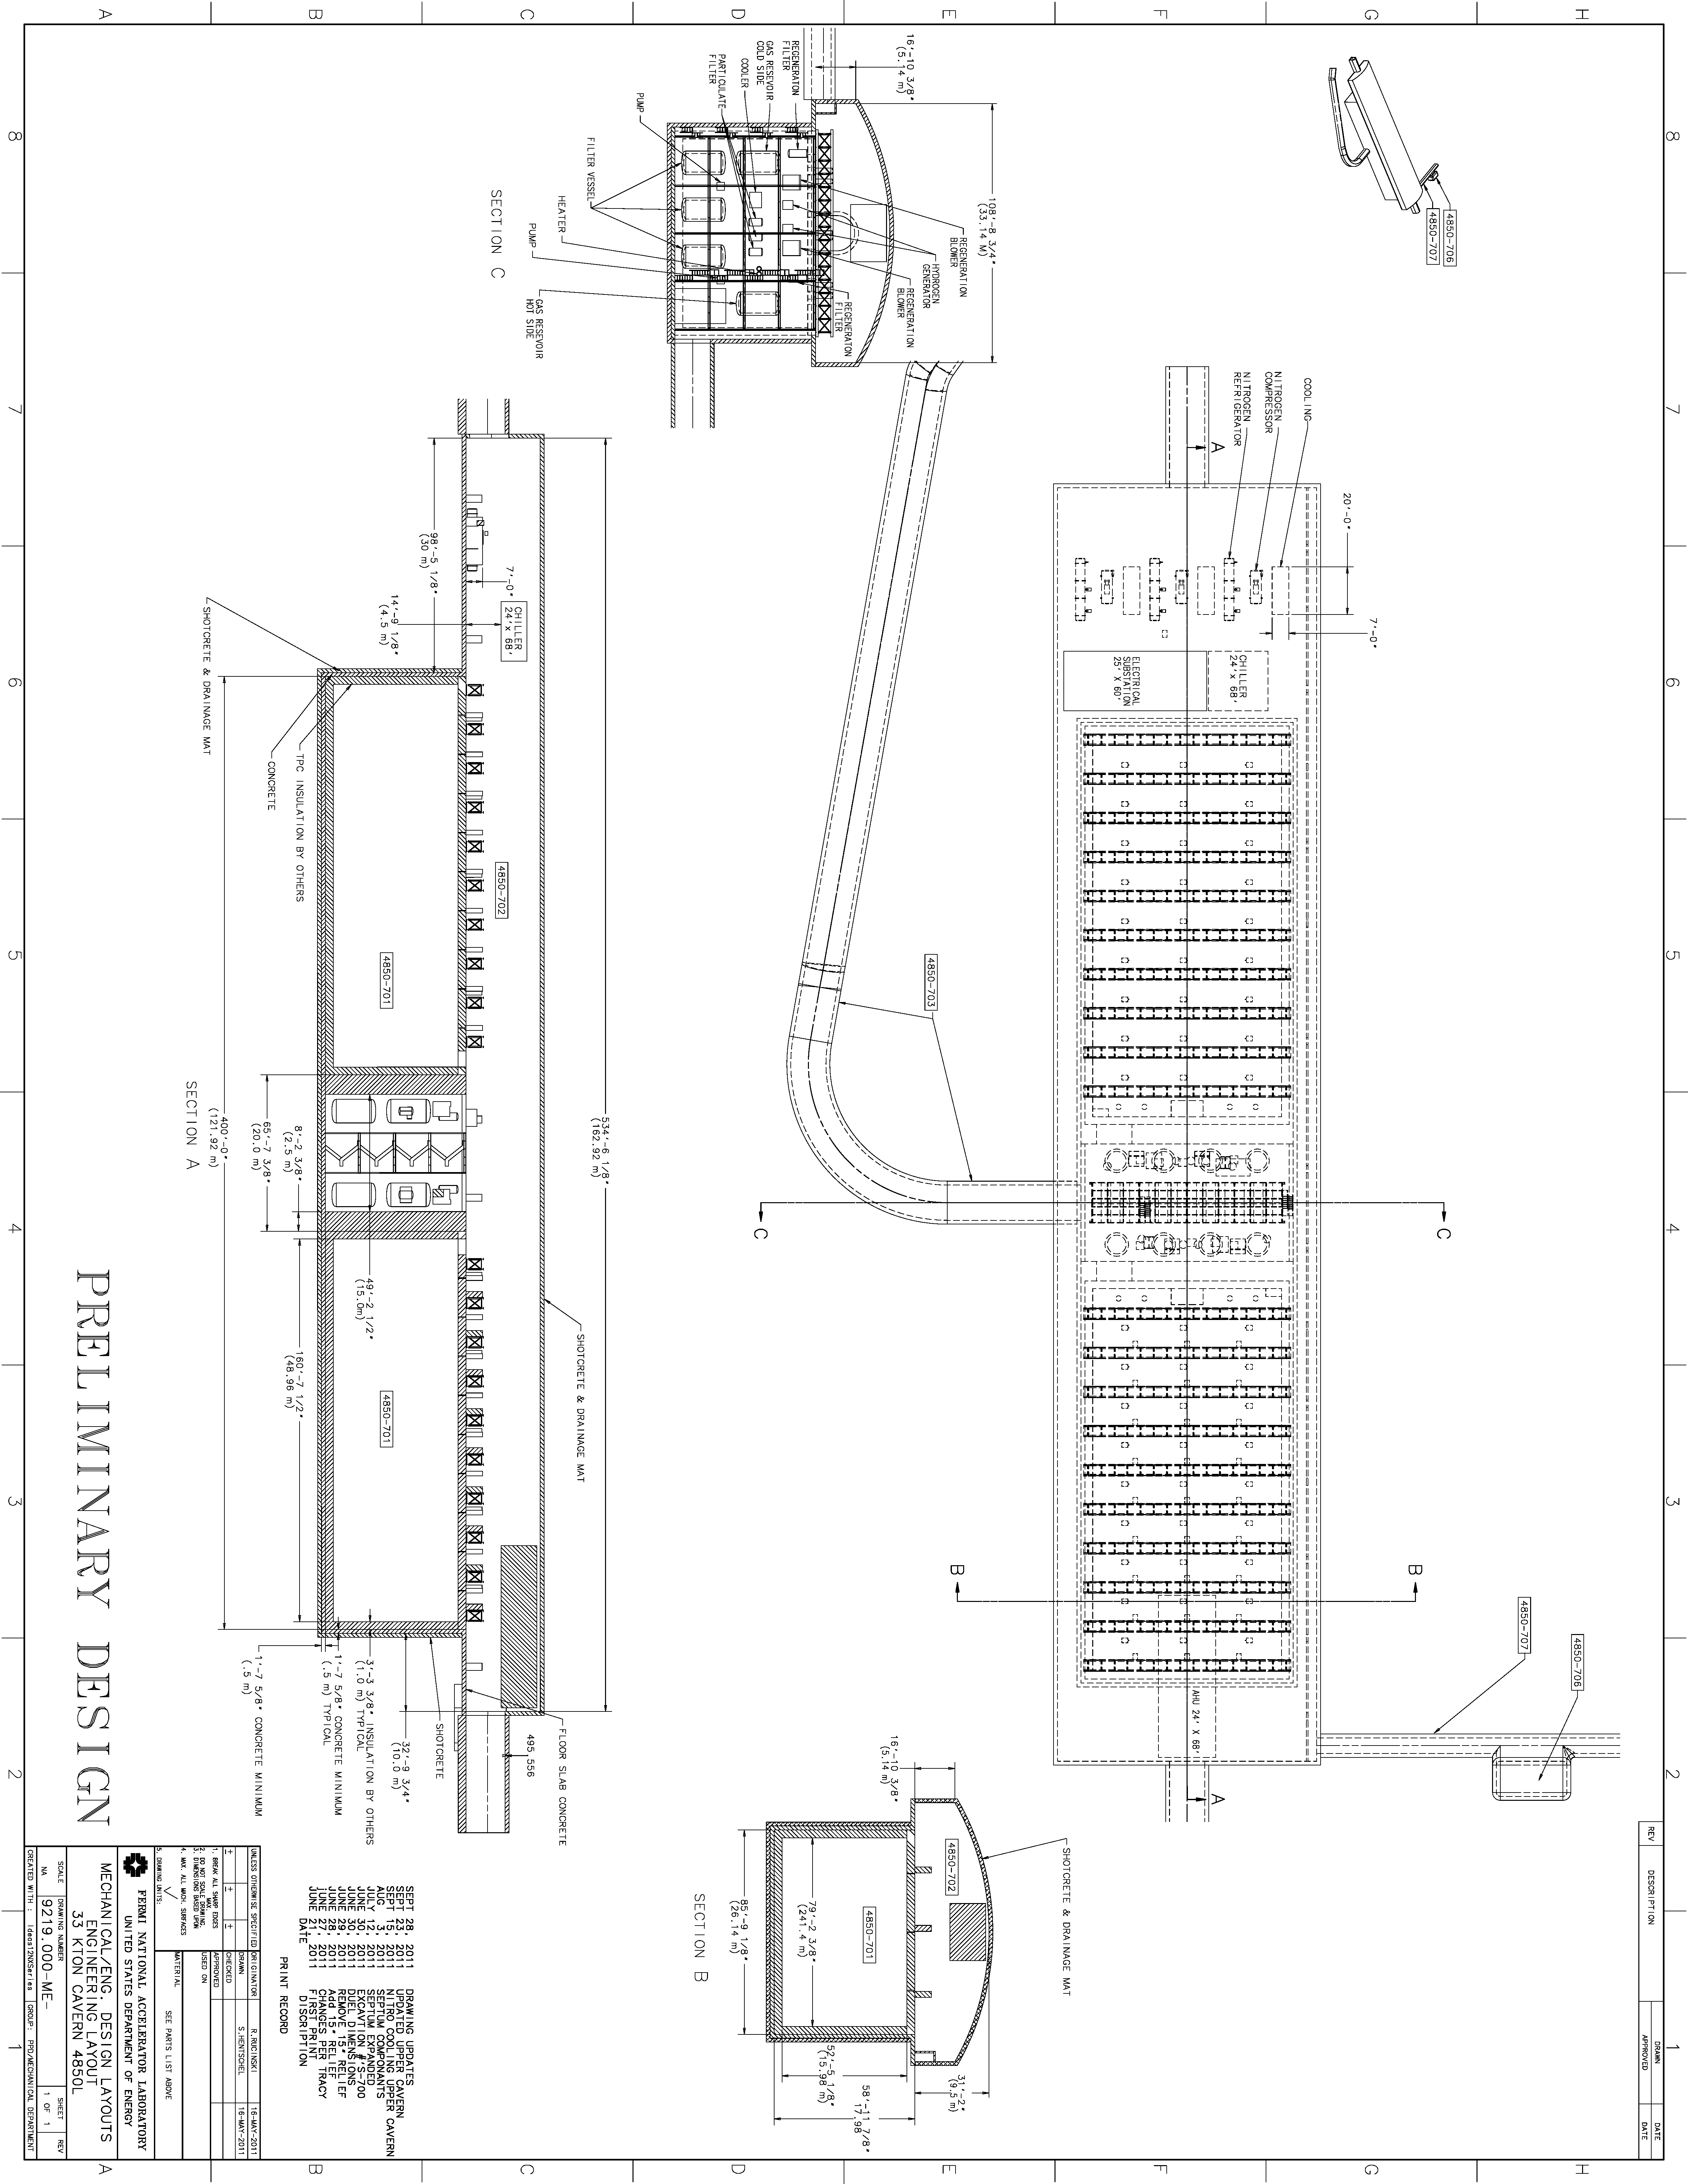
\includegraphics[width=\textwidth, angle=180]{v5ch2-4850-cavern-cryostat-dimensions}
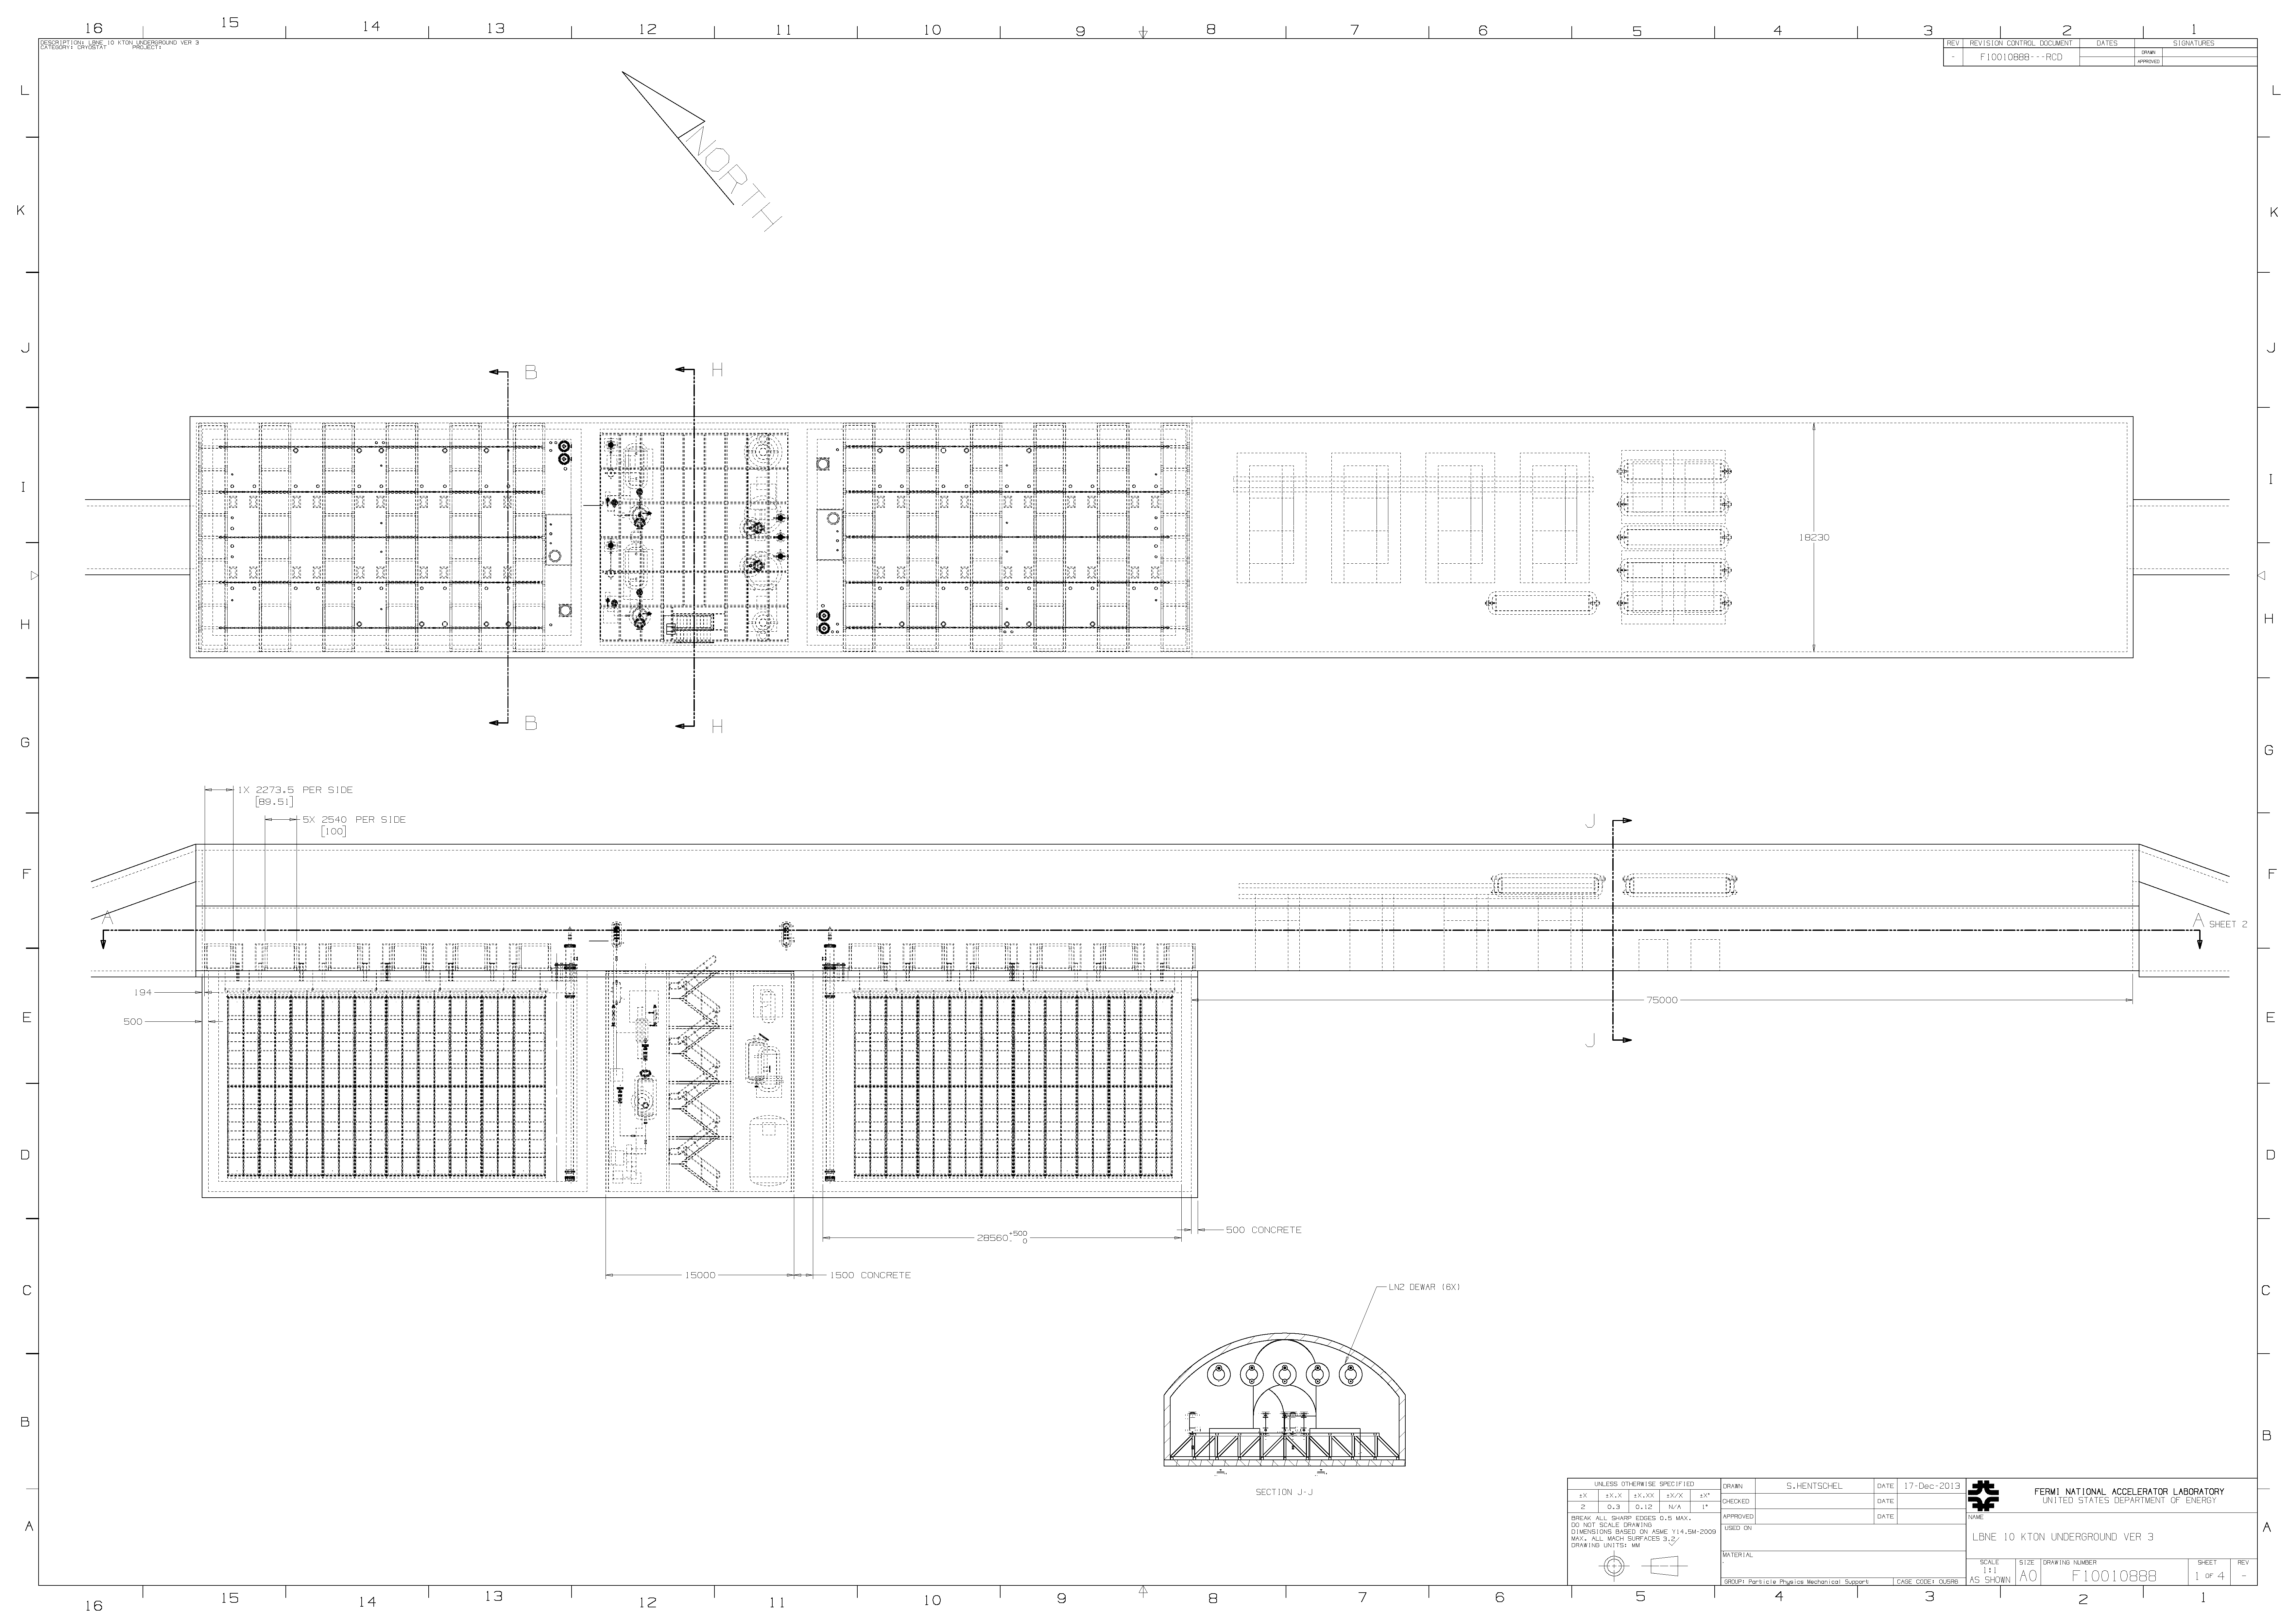
\includegraphics[width=\textwidth, angle=90]{F10010888--sht1--optim.png}
\caption[Dimensions for 10-kton detector cavern and cryostat, 2014]{Dimensions for 10-kton detector cavern 
and cryostat, 2014. The left-hand figure is a top view of the cavern hall; on the right is an elevation view 
through the cryostat and highbay. 
}
\label{fig:v5ch2-cavern-cryostat-section-2014}
\end{figure}


\subsection{Cryostat Construction}
\label{ch1:cryo-constr}
%added from ch 2, 2/23/12

The 10-kton cryostat construction uses commercial stainless-steel membrane technology engineered and produced by 
industry. These vessels are widely deployed in liquefied natural gas (LNG) tanker ships and 
tanks, and are typically manufactured in sizes much larger than that of the LAr-FD.  This is an inherently clean technology with passive insulation.

The LAr-FD cryostat reference design was selected on the recommendation of the experienced engineering consultants from ARUP USA, Inc.~\cite{docdb4314} after consideration of an alternative design that uses segmented, internally self-supporting, evacuable, modular cryostats.  Evacuation, in particular, appears not to be necessary; in September 2011, the Fermilab Liquid Argon Purity Demonstrator (LAPD)  achieved
 purity levels of less than 100 ppt oxygen-equivalent, using the method that is planned for use in the LAr-FD. This confirms that the 
method works, obviating the risk to LBNE that an evacuable vessel will be
 required. Operation of a 35-ton prototype using membrane-cryostat technology has provided a further demonstration.

The LAr-FD membrane cryostats are sealed containers supported by the surrounding rock.  This ``in-ground'' configuration offers access only from the top and protects against possible cryogen leaks out of the tank. The side walls consist of a series of membranes, foam insulation and reinforced concrete poured against the shotcrete covered rock. The inner (primary) membrane liner, made of stainless steel, is corrugated to provide strain relief from temperature-related expansion and contraction. 

%%%%%%%%%%%%%%%%%%%%%%%%%%%%%%%%%%%%%%%%%%%%%%%%%%%%%%%%%%%%%%%%%%%%%%

\subsection{Cryogenic Systems}
\label{sec:det_cryogenics}

Cryogenic systems are needed to manage the LAr, i.e., to keep it cold, pure and circulating smoothly during operations in order to maintain a sufficiently long drift lifetime for the ionization electrons. The major cryogenic systems used to perform these functions are the cryogen supply for cool-down and fill, gas filtration, argon condensing, liquid filtration and circulation and argon purity analysis.

The overall cryogenic system's layout and location is intended to optimize safety and efficiency. It is designed to minimize:
\begin{itemize}
\item the risk of personnel injury to any Oxygen Deficiency Hazard (ODH) 
\item heat ingress to the cryogenic system (by minimizing piping length and pump power)
\item the volume of the argon system external to the cryostat and hence the potential for argon escape or contamination
\end{itemize}
It is also designed to provide safe access to refrigeration equipment that requires periodic maintenance.

Cryogenic systems are located on the surface and within the cavern.  
Figure~\ref{fig:eqp-at-surface}  illustrates the cryogenic systems layout, which is described in 
Section~\ref{sec:cryosys-layout}.
%The re-condensers and purifiers will be located underground, adjacent to the cryostat. 

The required flow rate of liquid argon to be sent for purification is expected to decrease over time.  The 
initial maximum flow rate will be 51~m$^3$/hr (224~gpm).  The liquid-argon volume in one cryostat will turn over every five days at this rate. 
 Longer term, the rate will decrease to 25~m$^3$/hr with a turn-over rate of 11 days.  As a point of comparison, ICARUS T600 has a maximum turn-over rate of eight to ten days.

\subsection{LAr Purification}

The purification of LAr is accomplished with standard industrial equipment, using molecular sieves and chemically reducing materials, which are scalable within the contemplated range to accommodate the estimated irreducible material-outgassing from warm materials in the vapor space above the liquid argon, called the ullage. 


\subsection{Time Projection Chamber}

The Time Projection Chamber (TPC) is the active detection element of the LAr-FD. The construction concept is  shown schematically in Figures~\ref{fig:tpc-concept} and~\ref{fig:cpa-apa-arrangement-2014}.  A TPC is located
 inside each cryostat vessel and is completely submerged in LAr at 89~K. Five planes line up across the width: three Cathode Plane Assemblies (CPA)  
 interleaved with two Anode Plane Assemblies (APA). These planes are oriented vertically and 
 parallel to the beamline such that the electric fields applied between them are perpendicular to the beamline.  The TPC's active volume within the cryostat  is 12~m high, 14~m wide and 30~m along  
 the beam direction. 
 
 A ``drift cell'' is associated with one APA and the two CPAs on either 
 side of it; it is 
 defined as the volume between the enclosed APA's two surrounding CPAs, and bordered by the CPAs' edges.  The maximum electron-drift distance between a CPA and an adjacent APA (half 
 of the drift cell) is 3.4~m. Both the CPAs and APAs measure 2.3~m along beamline dimension and 6~m
 in height; they are each a few cm wide. 
 
 Each row of CPAs and APAs is 
 stacked two-high to instrument the 12-m active depth. Each row contains 13 such stacks placed edge-to-edge along the beam direction, forming the 30-m
 active length of the cryostat's TPC and resulting in a total of 52 APAs and 78 CPAs per cryostat. A ``field cage'' surrounds the top and ends of the cryostat to ensure uniformity of the electric field. The field cage is assembled from
 panels of FR-4 sheets with parallel copper strips connected to resistive divider networks.

Each APA has three wire planes that are connected to readout electronics; two induction planes (labeled U and V in Figure \ref{fig:tpc-concept}) and one collection plane (X). A fourth wire plane, grid plane (G), is held at a bias voltage but is not instrumented with readout electronics. The grid plane improves the signal-to-noise ratio on the U plane and provides electrostatic discharge protection for the readout electronics.

\begin{figure}[htbp]
\centering
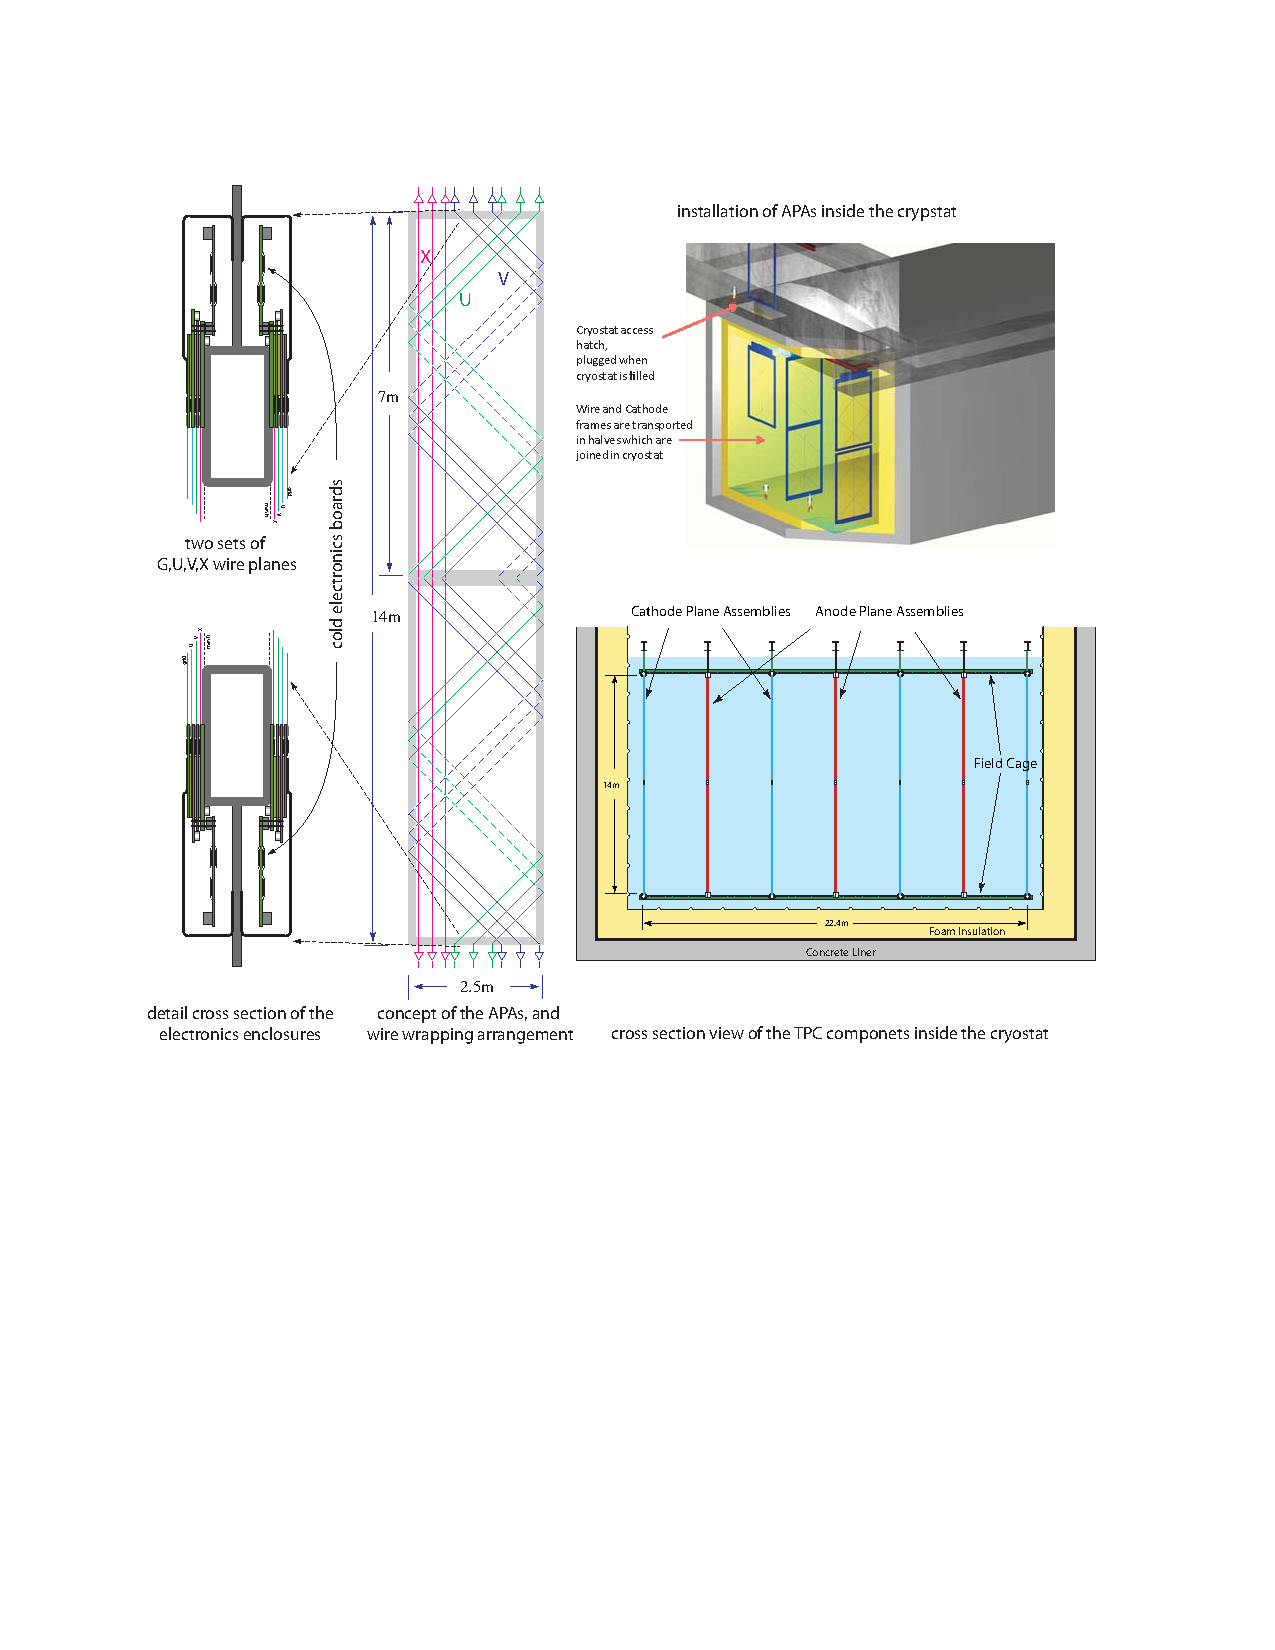
\includegraphics[width=\linewidth]{TPC_summary_figure}
\caption{TPC modular construction concept; the APA and CPA arrangement has been changed to two APAs and three CPAs as of 2014, see Figure~\ref{fig:cpa-apa-arrangement-2014}.}
\label{fig:tpc-concept}
\end{figure}

\begin{figure}[htbp]
\centering
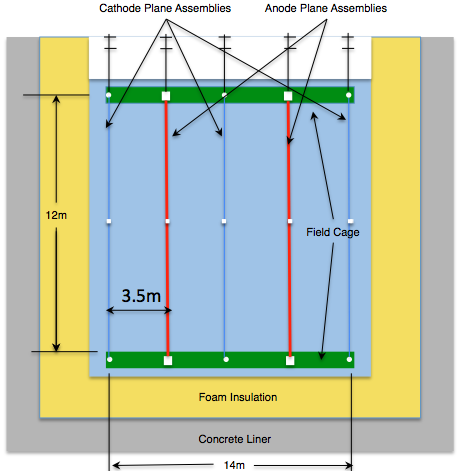
\includegraphics[width=\linewidth]{cpa-apa-arrangement-2014.png}
\caption{APA and CPA arrangement, 2014}
\label{fig:cpa-apa-arrangement-2014}
\end{figure}


\subsection{Electronics, Readout and Data Acquisition}
\label{sec:det_electronics}

CMOS technology, with a noise minimum at 89~K,
permits the front-end electronics to reside in the LAr (henceforth ``cold electronics''),
as close to the anode wires as is practical.
This minimizes capacitance and therefore signal noise,
and benefits LAr purity by not residing in the ullage gas.
Figure~\ref{fig:elect_schem_intro_copy} shows the cold electronics architecture,
which comprises a front-end shaping/filtering stage (FE ASIC),
an analog-to-digital conversion stage (ADC ASIC), and a communication/control stage (digital ASIC).
The signal feedthroughs are all located on top of the cryostat, where they are most accessible,
are at low hydrostatic pressure, and pose no risk of LAr leakage.
The cold electronics multiplex at 1:32,
which lowers the cable-count to what can be accomodated by the planned number of feedthroughs,
and mitigates contamination from cable outgassing
by reducing the volume of cables in the ullage gas.

% This is a copy of a figure which also appears in the CE chapter.
\begin{figure}[htbp]
\centering
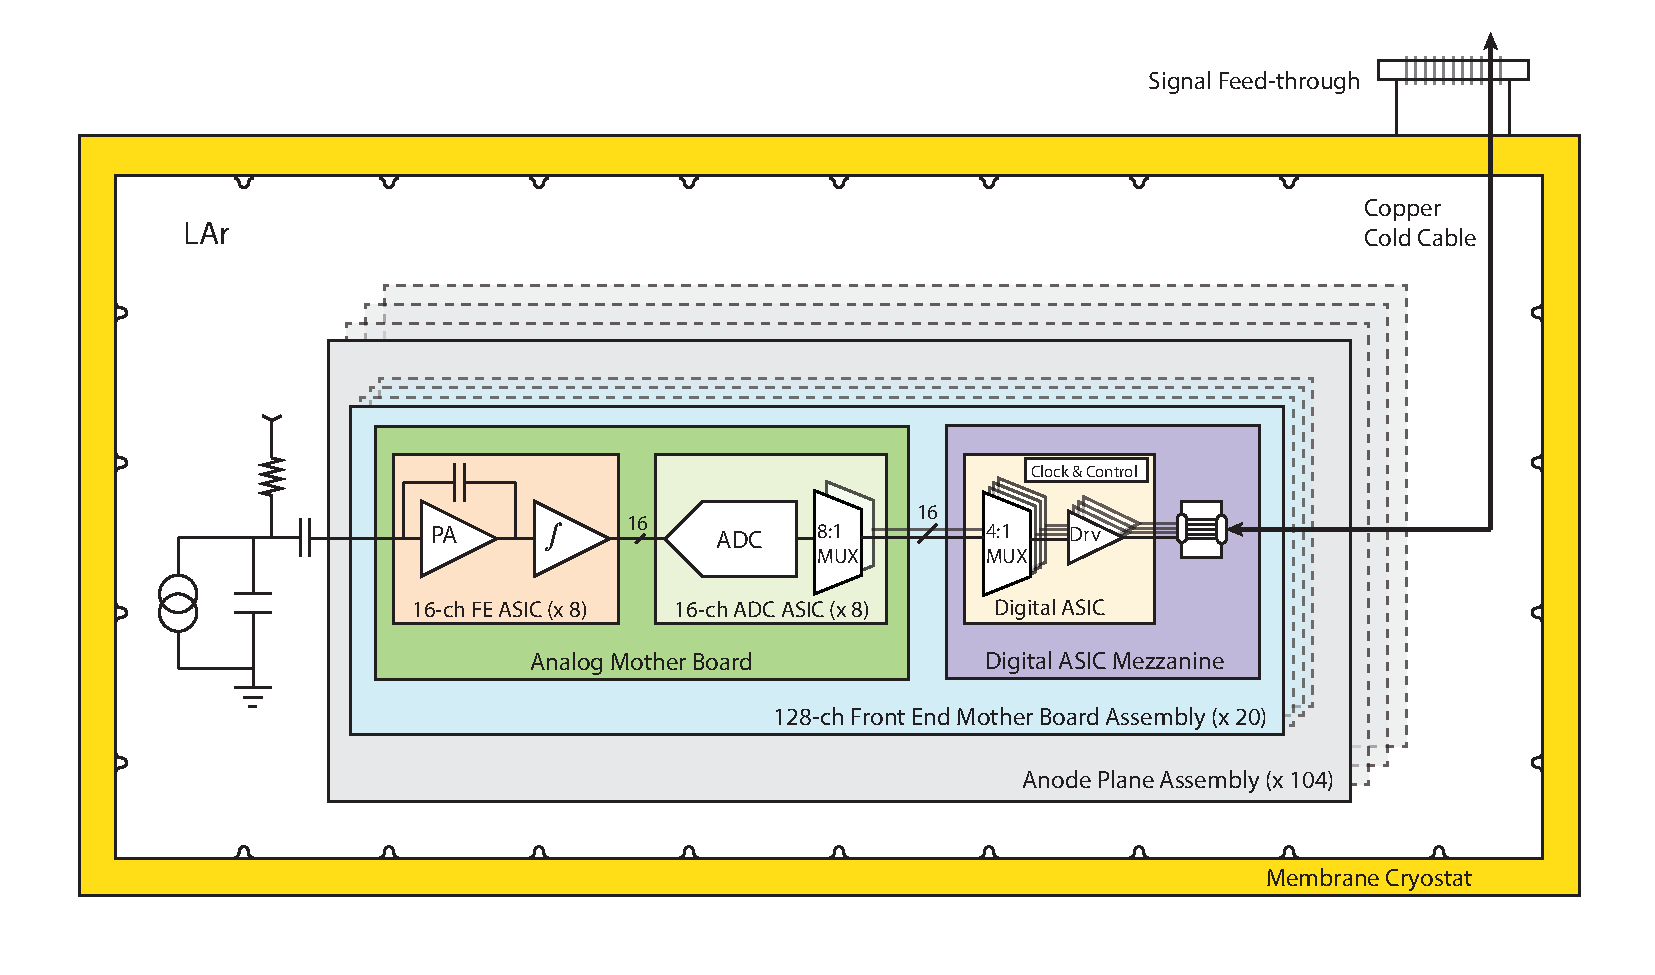
\includegraphics[width=\linewidth]{elect_schem.pdf}
\caption{Front-end electronics architecture.
         The ADCs multiplex at 8:1, while the digital ASICs multiplex at 4:1, together giving 32:1.
        }
\label{fig:elect_schem_intro_copy}
\end{figure}

%%%%%%%%%%%%%%%%%%%%%%%%%%%%%%%%%%%%%%%%%%%%%%%%%%%%%%%%%%%%%%%%%%%%%%


%%%%%%%%%%%%%%%%%%%%%%%%%%%%%%%%%%%%%%%%%%%%%%%%%%%%%%%%

\subsection{Photon-Detection System}

Identification of the different possible charged-particle types 
depends on accurate measurements of ionization along tracks. This requires accurate determination
of the time of interaction, or event time, $t_0$, which leads to the absolute location 
of the event along the drift axis, and allows the determination of $Q_0$,  the 
true ionization charge.

For non-accelerator physics events, $t_0$ is not known a priori.  
However, LAr is an excellent scintillator, generating of 
order $10^{4}$ 128-nm photons per MeV of deposited energy.  
Detection of scintillation photons 
provides a prompt signal that allows unambiguous 
location of particle positions along the drift axis.

The reference design for the photon detection system is based on acrylic bars, which are either coated in TPB or doped in bulk. The 128 nm photons interact with the TPB on the surface and 430 nm light is re-emitted. 
%The photon-detection system consists of acrylic light-guides that lead to SiPMs, as shown in Figure~\ref{fig:lightGuideProto}. Approximately 5\% of the converted photons incident on a light guide are captured within it and travel to the PMT. A wavelength-shifting coating on the light guides efficiently converts the scintillation photon wavelength from 128~nm to 428~nm where the PMT is most sensitive.  The fast PMT 
The signals will be routed out of the cryostat to standard readout electronics.

Twenty light-guide and SiPM assemblies, or ``paddles'', will be installed within each APA frame prior to wire winding. The SiPM signals will be used as a software ``trigger'' in the DAQ to define the event time, t$_0$, for non-accelerator events. This system provides a $t_0$ signal throughout the entire detector in contrast to a system similar to that used in MicroBooNE and ICARUS, where light is detected outside the detector volume. 

%%%%%%%%%%%%%%%%%%%%%%%%%%%%%%%%%%%%%%%%%%

\subsection{Detector Installation and Operation}
\label{sec:det-install}

Detector components will be shipped in sealed containers to the Far Site by truck and lowered to the cavern. Shipping containers will be moved to a clean area over the septum area between the cryostats. There the components will be unpacked from the sealed container and lowered  through an access hatch into the cryostat. 

The construction of the two cryostats and the installation and commissioning activities will
be staged such that both TPCs can be tested cold while one cryostat still remains available
as a potential LAr storage vessel. The LAr in one cryostat can be transferred to the other, and
back again, if necessary, until all the tests complete successfully. Once both TPCs are known to work properly at LAr temperature, the second fill will take place.

To protect the membrane on the floor of the cryostat during TPC installation, a temporary floor will be installed. 
After each pair of APAs is installed, they will be connected to the DAQ system and the wire integrity tested. All wires on previously installed APA pairs will also be tested. The wire integrity test will be performed during cryostat cool-down as well. A relatively slow cool-down rate will ensure that the temperature-induced stresses in the APA frames and wires are kept well below the level experienced during testing. 

An installation and integration detector mock-up will be constructed at Fermilab to confirm that interfaces between detector systems are well defined and to refine the installation procedures. 

%%%%%%%%%%%%%%%%%%%%%%%%%%%%%%%%%%%%%%%%%%%%%%%%%%%%%%%%%%%%%%%

\section{Principal Parameters}

The principal parameters of the LAr-FD are given in Table~\ref{table:param-summ-larfd}. 

\begin{table}[htpb]
\caption{LAr-FD Principal Parameters for 10-kton Detector}
\label{table:param-summ-larfd}
\centering
 \begin{tabular}[htbp]{|l|| p{6cm} |}
\hline
Parameter & Value  \\
\hline\hline
Active (Fiducial) Mass &   13.8 (10.2)~kton \\
\hline
Number of Detector Modules (Cryostats) &  2 \\
\hline
Drift Cell Configuration within Module &  2~wide $\times$ 2~high $\times$ 13~long \\
\hline
Drift Cell Dimensions  &  2 $\times$ 3.4~m wide (drift) $\times$ 6~m high $\times$ 2.3~m long \\
\hline
Detector Module Dimensions &  14~m wide $\times$ 12~m high $\times$  30~m long \\
\hline
Anode Wire Spacing &  $\sim$4.8~mm \\
\hline
Wire Planes (Orientation from vertical) & Grid (0$^\circ$), Induction 1 (36$^\circ$), Induction 2 (-36$^\circ$), Collection (0$^\circ$) \\
\hline
Drift Electric Field &  500~V/cm \\ 
\hline
Maximum Drift Time & 2.1~ms \\
\hline
\end{tabular} 
\end{table}

\subsection{Design Considerations}

TPCs operated to date have been constructed with an anode wire spacing in the range of 3~mm (ICARUS) to 4.8~mm (Fermilab cosmic-ray stand). The amount of ionization charge collected on the wires increases with larger wire spacing, resulting in a better signal-to-noise ratio without serious consequences (the radiation length of LAr is $\sim$~30 times larger than the typical wire spacing). The electron-$\pi^0$ separation efficiency of a TPC with 5-mm wire spacing is only a few percent lower than one with 3-mm wire spacing. It is also clear that a TPC with larger wire spacing requires fewer wires and readout channels, resulting in lower cost. % could put this later

Only two wire planes are required to reconstruct events in three dimensions, however three wire planes will be implemented to provide N+1 redundancy. The third will improve the pattern-recognition efficiency for a subset of multi-track events in which trajectories can overlap in two views. The collection-plane wires are most commonly used for calorimetric reconstruction and are oriented vertically ($0^\circ$) to minimize both the wire length and the electronics noise.

\begin{editornote}
  Editor's Note:  The following paragraph refers to a wire orientation of 45 degrees.  The chosen wire orientation has been changed to 35.7 degrees from vertical.  The study and documentation justifying this choice is in LBNE-docdb-9374.
\end{editornote}


A study of wire orientation has shown that for a TPC with three instrumented wire planes, the optimum orientation of the induction plane wires should be between $\pm40^\circ$ and $\pm60^\circ$ when the collection plane wires are at $0^\circ$. The ideal orientation for the more isotropic low-energy events, e.g., 
supernova-neutrino interactions, is $\pm60^\circ$. The selected induction-plane wire orientation of $\pm45^\circ$ has better position resolution in the vertical direction than $\pm30^\circ$ and has shorter wires compared to a wire orientation of $\pm60^\circ$.  The induction plane wires are wrapped around the APA frames so that the readout electronics can be located on the top or bottom of the TPC. As a result, it is natural to arrange the APAs vertically in a two-high configration. 

  Access to the top of the cryostat is required to install and connect cabling. Therefore, risk of personnel injury and detector damage, both of which increase with height, form the primary considerations for the the detector height, 12~m. The  The height of the APA has been chosen, accordingly, to be 6~m, resulting in 6-m-long collection-plane wires and 7.3-m-long induction plane wires. 

The 2.3~m width of the APA was chosen to facilitate construction and to allow standard, over-the-road transport. 

The choice of cryostat width is based on the desired cryostat shape and cavern span. From a cryogenics standpoint, the ideal cryostat for a modular TPC would be a cube since membrane-cryostat capital and operating costs scale linearly with the surface area. This shape is not ideal for cavern excavation, however. In the absence of a geotechnical investigation for the cavern location, the cavern span has been limited to $\sim$30~m on the advice of rock engineers. A detector width of 14~m results after making allowance for cryostat insulation, and personnel access both above and within the cryostat. 

A drift field of 500~V/cm was chosen based on experience from similar detectors such as ICARUS, ArgoNeuT and the Fermilab cosmic-ray test stand. At this electric field, $\sim$ 30\% of the ionization electrons produced by the passage of a minimum ionizing particle (MIP) recombine and create scintillation light that provides a fast trigger. The remaining ionization electrons drift to the APA and produce wire-plane signals. The TPC could function at higher or lower drift fields but the relative yields of scintillation light and ionization electrons would change. The use of a higher drift field would require more care in the design of the high-voltage systems. The electron drift velocity is 1.6~mm/$\mu$s at 500~V/cm.

The 14~m width of the the detector can be divided into four drift cells with a maximum drift length of 3.41~m each. This drift cell length was chosen based on experience from other detectors, the required minimum signal-to-noise ratio and high-voltage considerations. The required minimum signal-to-noise ratio of 9:1 ensures that the tracking efficiency will be 100\% throughout the entire drift cell. The TPC must be capable of detecting the smallest signal (1~MeV) produced in interactions that LBNE will study. This situation occurs when a MIP travels parallel to a wire plane and perpendicular to the orientation of the wires in the plane. A MIP loses 2.1~MeV of energy in each cm of travel, producing $\sim$ 40,000 ionization electrons along every 5~mm section of the track. About 28,000 electrons escape recombination and, ignoring the effects of LAr purity and diffusion, would all drift to one collection plane wire. The capacitance due to the maximum-length 7.3~m wire is 164~pF resulting in an equivalent noise charge (ENC) of 500 electrons in the CMOS amplifiers. The signal-to-noise ratio would therefore be 53:1 if all of the ionization electrons arrived at the wire. For a maximum drift distance of 3.41~m and a drift field of 500~V/cm, the required voltage on the cathode plane is 173~kV. This is within the range of commercially available high-voltage cables and within the range of current designs for cryogenic feedthroughs. Additional R\&D would be needed for longer maximum drift lengths.

Ionization electrons will be lost due to impurities in the LAr. The fraction that survive passage to the anode planes is $e^{t/\tau}$, where$t$ is the drift time and $\tau$ is the drift-electron lifetime. The maximum drift time is the maximum drift length divided by 1.6~mm/$\mu$s which equals 2.3~ms for LBNE. The ICARUS detector has achieved a drift electron lifetime of 6 -- 7~ms. The Materials Test Stand (described in Section~\ref{sec:mts}) regularly achieves a drift-electron lifetime of 8 -- 10 ms. The Fermilab Liquid Argon Purity Demonstrator achieved a liftime of $>$ 3~ms during initial tests. Based on this experience, and by careful selection of materials in the ullage,  a drift-electron lifetime at least as good as ICARUS is expected. The signal-to-noise ratio would be 36:1 for a drift electron lifetime of 6~ms. A minimum lifetime of 1.4~ms is required to meet the 9:1 signal-to-noise ratio requirement.

The cloud of drifting ionization electrons will spread out in space due to the effects of diffusion. The maximum transverse $RMS$ width of the electron cloud is 2.4~mm for the chosen drift distance and drift field. This is well matched to the 5~mm wire spacing.

\section{Detector Development Program}

As mentioned above, the design of the LAr-FD has benefited greatly from other experiments and related development activities. Development activities in the U.S. are described in the  {\em Integrated Plan for LArTPC Neutrino Detectors in the US}~\cite{IP}. This program includes non-LBNE activities such as the Fermilab Materials Test Stand, Fermilab electronics test stand, LAPD, photon detection, ArgoNeuT and MicroBooNE as well as LBNE activities such as the 35-ton prototype and LAr1. The development plan is described in detail in Chapter \ref{ch:randd}.


\begin{editornote}
  Editor's Note: The far detector prototyping plan known as LAr1 has been replaced by a plan to build and test a prototype with full-size TPC components at CERN.
\end{editornote}


\section{Participants}

The design for the LBNE Far Detector is being carried out by an LBNE subproject team, headed at Fermilab  but with participants also from Brookhaven National Laboratory, Argonne National Laboratory and Indiana  University, in conjunction with an engineering design firm, Arup USA, Inc.  This firm has assisted with cryostat and cryogenic-plant design.  The detector is planned for construction at the  Sanford Laboratory site, which is managed by the South Dakota Science and Technology Authority  (SDSTA).

The LBNE Far Detector, called the LAr-FD, is managed by the Work Breakdown Structure (WBS)  Level 2 Manager for the Far Detector subproject. The supporting team includes a WBS Level 3  Manager for each of its component systems: Cryogenics \& Cryostat, Time Projection Chamber (TPC),  Trigger \& Data Acquisition (DAQ), Installation \& Commissioning and Photon Detector.  Figure~\ref{fig:lar-org} shows an organization chart down to Level 3 (L3).

\begin{figure}
\begin{center}
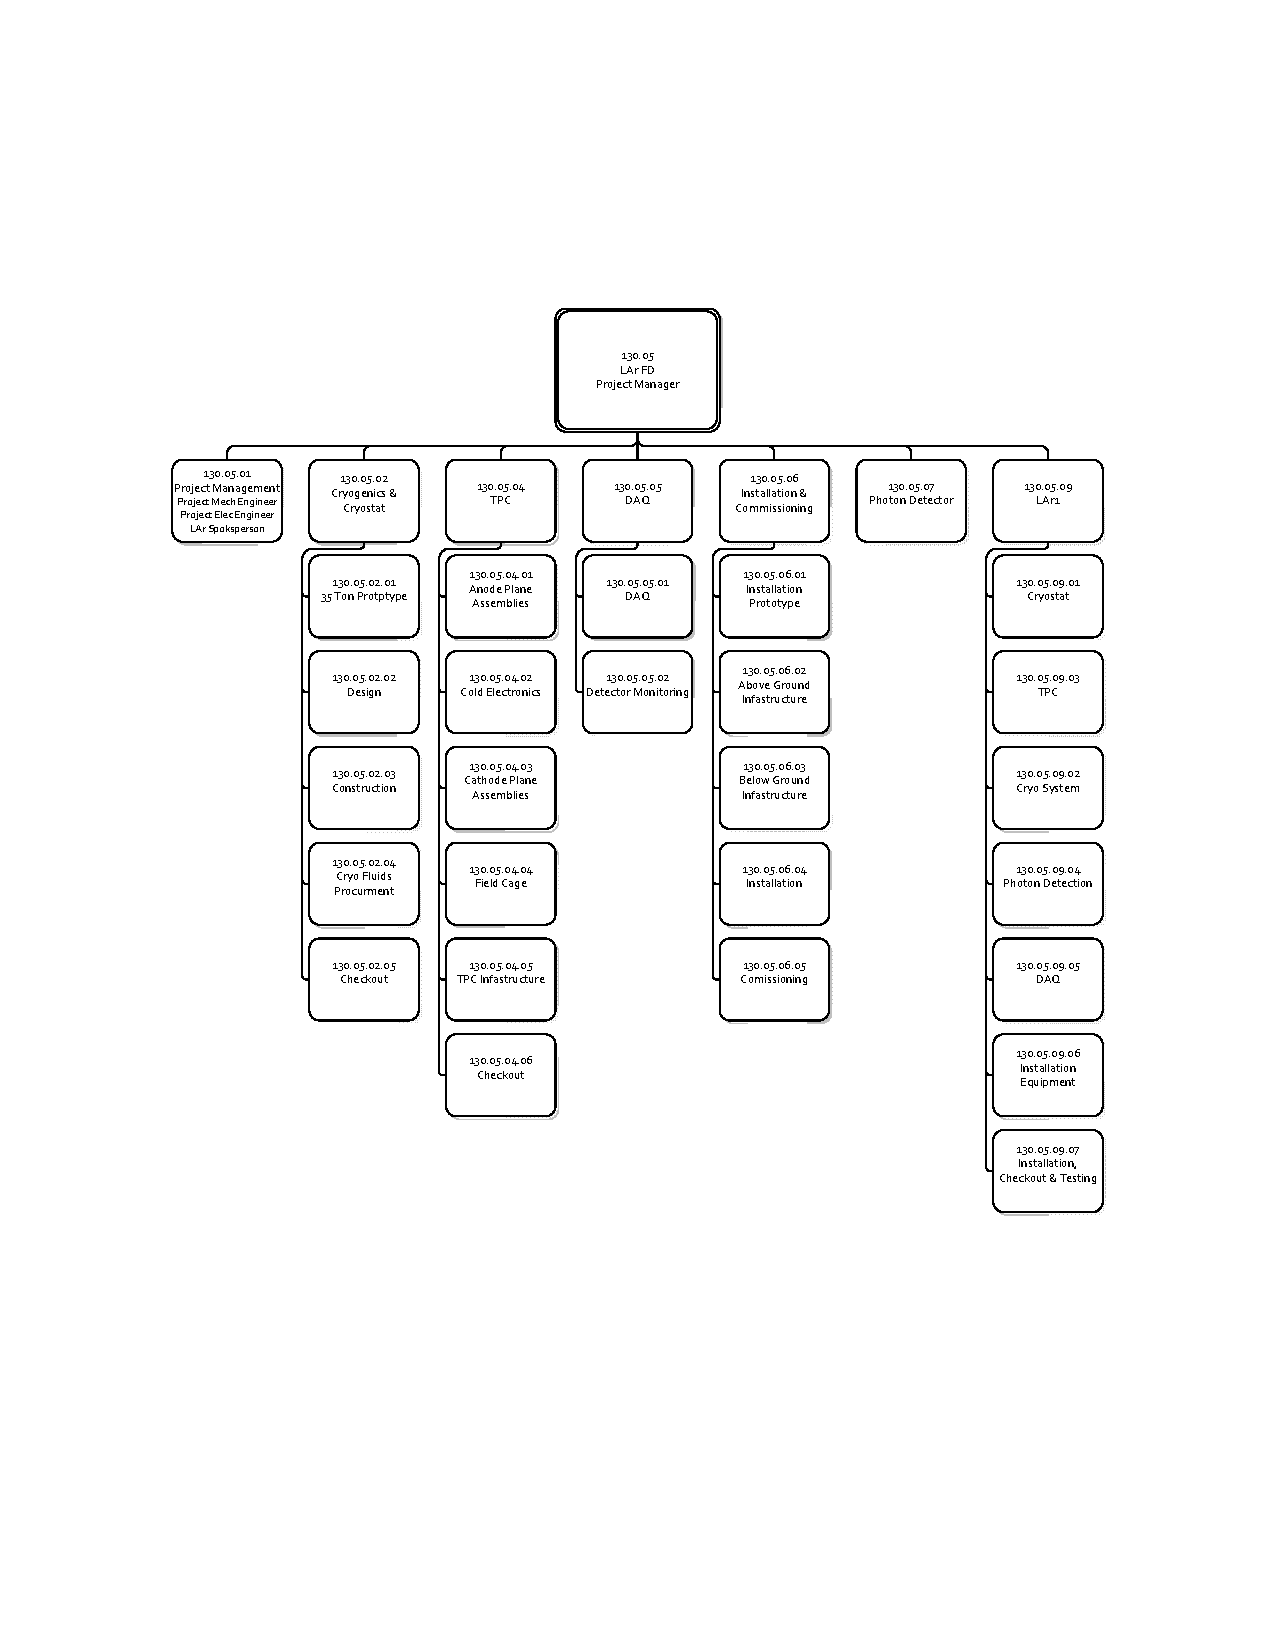
\includegraphics[width=.9\textwidth]{lar-org-chart-nonames}
\caption[Organization chart for the Far Detector subproject]{\label{fig:lar-org} Organization chart for the Far Detector subproject (as of 2012)}
\end{center}
\end{figure}

The Conventional Facilities Level 3 Far Site Manager is the LBNE Project liaison with the LAr-FD subproject  to ensure the detector requirements are met; this person is responsible for all LBNE scope at the Far Site.  [Management of the Sanford Lab and the organizational relationship between it and the LBNE Project and  Fermilab are in the process of being determined; this section will be updated when that is known.]

\nomenclature{ADC}{analog-to-digital converter}
\nomenclature{APA}{anode plane assembly}
\nomenclature{APD}{avalanche photodiodes}
\nomenclature{ArgoNeuT}{Mini LArTPC Exposure to Fermilab's NuMI Beam}
\nomenclature{ASIC}{application-specific integrated circuit}
\nomenclature{BGR}{band-gap reference}
\nomenclature{CAD}{computer-aided design}  
\nomenclature{CDF}{one of two decommissioned collider detectors at Fermilab's Tevatron, along with D-Zero}  
\nomenclature{CF}{conventional facilities} 
\nomenclature{CFD}{computerized fluid dynamics} 
\nomenclature{CPA}{cathode plane assembly}
\nomenclature{DAQ}{data acquisition}
\nomenclature{DCM}{data concentrator module}
\nomenclature{DC}{direct current}
\nomenclature{DCM}{Data concentrator modules}
\nomenclature{D-Zero}{one of two decommissioned collider detectors at Fermilab's Tevatron, along with CDF}
\nomenclature{EM}{electromagnetic}
\nomenclature{ENC}{equivalent noise charge}
\nomenclature{ESH}{Environment, Safety and Health}
\nomenclature{FEM}{front-end module}
\nomenclature{FESHM}{Fermilab's ES\&H Manual}
\nomenclature{FFT}{Fast Fourier Transform}
\nomenclature{FIRUS}{Fire and Utilities; Fermilab site-wide, high-reliability, remote monitoring system used to monitor building fire panels and various utilities throughout the lab}
\nomenclature{FLARE}{Fermilab Liquid Argon Experiments}
\nomenclature{FPGA}{field-programmable gate array}
\nomenclature{FR-4}{flame resistant 4}
\nomenclature{FSE}{field-shaping electrode}
\nomenclature{GAr}{gaseous argon}
\nomenclature{GLACIER}{NASA's General Laboratory Active Cryogenic International Space Station Experiment Refrigerator}
\nomenclature{LNGS}{Gran Sasso National Laboratory}
\nomenclature{G10/FR4}{a fire rated electrical-grade dielectric made with and epoxy material reinforced with a woven fiberglass mat}
\nomenclature{GTT}{Gaztransport \& Technigaz}
\nomenclature{HSSD}{High Sensitivity Smoke Detection}
\nomenclature{HV}{high voltage}
\nomenclature{HVAC}{heating, ventilation and air conditioning}
\nomenclature{ICARUS}{Imaging Cosmic and Rare Underground Signals, experiment at the LNGS}
\nomenclature{INFN}{Istituto Nazionale della Fiscia Nucleare} 
\nomenclature{IHI}{Ishikawajima-Harima Heavy Industries}
\nomenclature{IT}{integration prototype}
\nomenclature{IU}{Indiana University}
\nomenclature{LANNDD}{Liquid Argon Neutrino and Nucleon Decay Detector}
\nomenclature{LAPD}{Liquid Argon Purity Demonstrator}
\nomenclature{LAr}{liquid argon}
\nomenclature{LAr1}{one-kiloton LAr prototype for LBNE's LAr-FD}
\nomenclature{LAr-FD}{LBNE's Liquid Argon Far Detector}
\nomenclature{LArSoft}{a reconstruction software package for LAr detectors}
\nomenclature{LArTPC}{liquid argon time projection chamber}
 \nomenclature{LBNE}{Long-Baseline Neutrino Experiment}
\nomenclature{LED}{light-emitting diode}
\nomenclature{LEM}{large electron multiplier}
\nomenclature{LEMO}{a push-pull connector made by the LEMO company in Switzerland}
\nomenclature{LHe}{liquid helium}
\nomenclature{LN}{liquid nitrogen, also written LN$_2$ and LN2}
\nomenclature{LNG}{liquefied natural gas}
\nomenclature{LOTO}{lockout/tagout; an OSHA safety practice }
\nomenclature{LPG}{liquefied petroleum gas}
\nomenclature{LVDS}{low-voltage differential signaling}
\nomenclature{MCT}{membrane cryostat test}
\nomenclature{MicroBooNE}{A 100-ton LArTPC located along Fermilab's Booster neutrino beamline }
\nomenclature{MINERvA}{A neutrino-scattering experiment that uses the NuMI beamline at Fermilab}
\nomenclature{MINOS}{Main Injector Neutrino Oscillation Search, a Fermilab experiment}
\nomenclature{MIP}{minimum ionizing particle}
\nomenclature{MIT}{Massachusetts Institute of Technology}
\nomenclature{MOS}{metal-oxide semiconductor}
\nomenclature{MOSFET}{metal-oxide-semiconductor field-effect transistor}
\nomenclature{MTU}{master timing unit}
\nomenclature{MUX}{multiplex}
\nomenclature{Bis-MSB}{1,4-bis[2-(2-methylphenyl)ethenyl]-benzene, a wavelength-shifting chemical}
\nomenclature{MTS}{Materials Test Stand}
\nomenclature{N or N2}{nitrogen}
\nomenclature{NASA}{National Aeronautics and Space Administration}
\nomenclature{NBTI}{negative bias temperature instability}
\nomenclature{NC}{neutral current}
\nomenclature{NICADD}{Northern Illinois Center for Accelerator and Detector Development NOvA}
\nomenclature{NIM}{Nuclear Instruments and Methods (journal)}
\nomenclature{NIST}{National Institute of Standards and Technology}
\nomenclature{NIST}{National Institute of Standards and Technology}
\nomenclature{NSF}{National Science Foundation}
\nomenclature{NOvA}{NuMI Off-Axis Neutrino Appearance experiment at Fermilab}
\nomenclature{OD}{outer diameter}
\nomenclature{ODH}{oxygen deficiency hazard}
\nomenclature{OPERA}{Oscillation Project with Emulsion-Racking Apparatus, at CERN and LNGS}
\nomenclature{OSHA}{Occupational Safety and Health Administration}
\nomenclature{PC}{personal computer}
\nomenclature{PC-4}{Fermilab building, Proton Center building number 4}
\nomenclature{PCI}{peripheral component interconnect}
\nomenclature{PDA}{photon detection assembly}
\nomenclature{PDE}{photon-detection efficiency}
\nomenclature{PE}{photo-electron}
\nomenclature{PLC}{programmable logic controller}
\nomenclature{PMT}{photomultiplier tube}
\nomenclature{PPE}{personnel protective equipment}
\nomenclature{PRV}{pressure-relief valve}
\nomenclature{QC}{quality control}
\nomenclature{RC}{resistive capacitive}
\nomenclature{ROOT}{An object oriented framework for large-scale data analysis developed at CERN}
\nomenclature{SCR}{silicon controlled rectifier}
\nomenclature{SDSTA}{South Dakota Science and Technology Authority}
\nomenclature{SIMOPS}{simultaneous operations study}
\nomenclature{SiPM}{Silicon photomultiplier}
\nomenclature{SM}{stress-migration}
\nomenclature{S/N}{signal-to-noise }
\nomenclature{SS}{stainless steel}
\nomenclature{TC}{thermal cycling}
\nomenclature{TDDB}{time-dependent dielectric breakdown}
\nomenclature{TDU}{timing distribution unit}
\nomenclature{TPB}{tetraphenyl butadiene, a wavelength shifting chemical}
\nomenclature{TPC}{Time Projection Chamber}
\nomenclature{USB}{universal serial bus}
\nomenclature{UV}{ultraviolet}
\nomenclature{VME}{a computer bus standard}
\nomenclature{VUV}{vacuum ultraviolet light}
\nomenclature{WARP}{Wimp Argon Program}
\nomenclature{WBS}{Work Breakdown Structure}
\nomenclature{WLS}{wavelength shifter}

\nomenclature{A}{ampere (also mA, kA)   }
\nomenclature{atm}{atmosphere}
\nomenclature{bar}{bar (also mbar, etc.)}
\nomenclature{barg}{bar gauge (deprecated per Wikipedia)}
\nomenclature{b}{barn, a measure of cross section; bit (also Mb, Gb, etc.)}
\nomenclature{B}{byte (also MB, GB, etc.)}
\nomenclature{Bq}{becquerel}
\nomenclature{C}{coulomb}
\nomenclature{cf}{cubic foot (also ft$^3$)}
\nomenclature{cfm}{cubic feet per meter (also ft$^3$/m)}
\nomenclature{Ci}{curie}
\nomenclature{eV}{electron-volt (also keV, MeV, GeV) }
\nomenclature{F}{farad (also pF, nF )}
\nomenclature{ft}{foot or feet }
\nomenclature{gal}{gallon}
\nomenclature{gpm}{gallons per minute (also gal/min)} 
\nomenclature{G}{gauss (also mG) or gradient (in magnets)}
\nomenclature{g}{gram (also mg, kg)}
\nomenclature{Hz}{hertz (s-1)}
\nomenclature{h}{hour}
\nomenclature{in}{inch }
\nomenclature{K}{kelvin} 
\nomenclature{l}{liter}
\nomenclature{m}{meter (also nm, micron, mm, cm, km) }
\nomenclature{min}{minute }
\nomenclature{MICA}{type of dielectric material used in capacitors}
\nomenclature{MS}{mega samples}
\nomenclature{N}{newton}
\nomenclature{NPO}{type of dielectric material used in capacitors}
\nomenclature{QFP}{quad flat pack}
\nomenclature{R}{roentgen}
\nomenclature{Pa}{pascal}
\nomenclature{psi}{pounds per square inch}
\nomenclature{rad}{radian (also mrad) }
\nomenclature{s}{second (also ns, $\mu$s, ms) }
\nomenclature{scfm}{standard cubic foot per minute }
\nomenclature{SHV}{safe high voltage, a type of HV cable connector}
\nomenclature{t}{ton}
\nomenclature{T}{Tesla}
\nomenclature{V}{volt (also mV, kV, MV)}
\nomenclature{VA}{volt-ampere (also mVA, kVA, MVA)}
\nomenclature{VAC}{Volts alternating current (also mVAC, kVAC)}
\nomenclature{VUV}{vacuum ultraviolet}
\nomenclature{W}{watt (also mW, kW, MW) }
\nomenclature{yd}{yard }
